\begin{frame}{Architecture}
    \begin{itemize}
        \item \mlblinkui (client): focuses in user interaction and experience
    \end{itemize}
\end{frame}

\begin{frame}{Architecture}
    \begin{itemize}
        \item \mlblinkui (client): focuses in user interaction and experience
        \item \mlblinkapi (server): domain logic and providing the required resources to the \mlblinkui
    \end{itemize}
\end{frame}

\begin{frame}{Architecture}
    \begin{itemize}
        \item \mlblinkui (client): focuses in user interaction and experience
        \item \mlblinkapi (server): domain logic and providing the required resources to the \mlblinkui
        \item Advantages: separation of concerns, support different types of clients, and easier delegation
    \end{itemize}
\end{frame}

\begin{frame}{Architecture}
    \begin{itemize}
        \item \mlblinkui (client): focuses in user interaction and experience
        \item \mlblinkapi (server): domain logic and providing the required resources to the \mlblinkui
        \item Advantages: separation of concerns, support different types of clients, and easier delegation
        \item Disadvantages: higher operational cost, complexity (cognitive load)
    \end{itemize}
\end{frame}


\begin{frame}{Architecture}
    \begin{figure}
      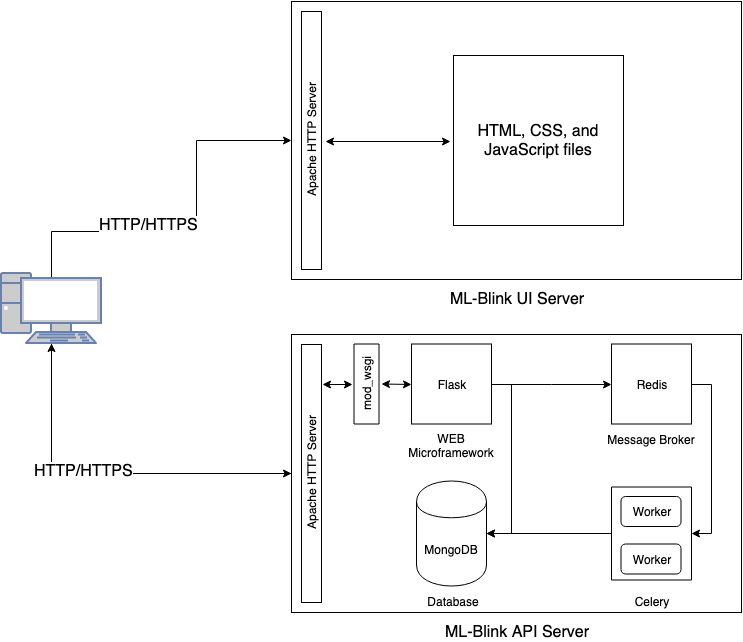
\includegraphics[
            height=0.8\textheight,
            keepaspectratio
      ]{report/images/ml-blink-architecture.png}
    \end{figure}
\end{frame}